%%This is a very basic article template.
%%There is just one section and two subsections.
\documentclass[a4paper, ngerman]{scrartcl}

\usepackage[T1]{fontenc}
\usepackage[utf8]{inputenc}
\usepackage[ngerman]{babel}
\usepackage{lmodern}
\usepackage{amsmath}
\usepackage{amsfonts}
\usepackage{hyperref}
\usepackage{graphicx}
\usepackage{paralist}
\usepackage[none]{hyphenat}
\usepackage{wrapfig}

\sloppy



\hypersetup{
pdfborder = {0 0 0},
urlbordercolor = {0 0 0},
colorlinks = true,
linkcolor = black,
citecolor = black,
filecolor = black,
urlcolor  = black
}

\title{Software-Challenge 2014 - Sixpack}
\subtitle{Spielregeln}



%% Variablen
\newcommand{\SpielFelderAnzahl}{\emph{256}}
\newcommand{\KartenAnzahl}{\emph{KartenAnzahl}}
\newcommand{\PiratenAnzahl}{\emph{6}}
\newcommand{\EmptyPlainPage}{\newpage\thispagestyle{plain}\ \newpage}
\newcommand{\RundenAnzahl}{\emph{15}}

\begin{document}
\parindent0px
\maketitle

\begin{figure}[h]
	\centering
	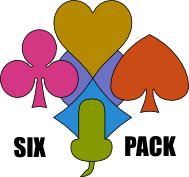
\includegraphics[scale = 1.0]{images/sixpack}
\end{figure}
\vspace*{\fill}

\newpage
\tableofcontents
\newpage

\section{Einführung}
In dieser Anleitung werden die Elemente und Regeln des Spiels \emph{Sixpack}
der Software-Challenge 2014 erläutert.\\
In dem Spiel versuchen zwei Spieler durch geschicktes Anlegen von Spielsteinen auf einem Spielbrett möglichst viele Punkte zu erlangen.

\section{Spielmaterial}
	\subsection{Das Spielbrett}
Das Spielbrett wird durch insgesamt \SpielFelderAnzahl\ Spielfeldern, welche in einer 16x16 Matrix angeordnet sind, gebildet. Die Nummerierung der Spielfelder beginnt dabei, wie in der Informatik üblich, bei 0. Jedes Spielfeld besitzt einen eindeutigen Index der sich aus x und y Koordinate, nach dem Schema (x,y), zusammensetzt. Das Spielfeld ganz links oben besitzt demnach den Index (0,0) (siehe Abbildung ~\ref{fig:Spielfeld}).\\

\begin{figure}[h] \centering 
	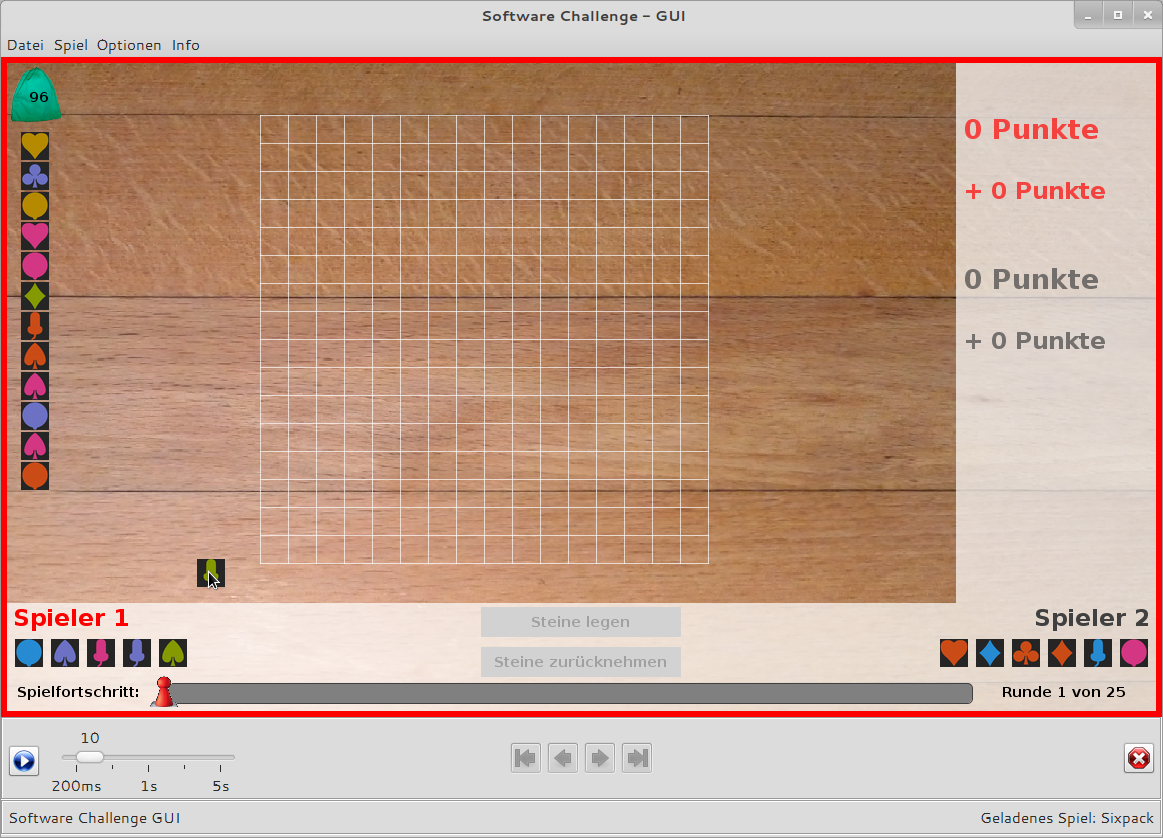
\includegraphics[scale = 0.3]{images/Spielbrett}
	\caption{Das Spielbrett.}
	\label{fig:Spielfeld}
\end{figure}

\subsection{Die Spielsteine}
Ein Spielstein besitzt eine von sechs möglichen Farben und eine von sechs möglichen Formen. Die sechs Farben sind \emph{Blau},\emph{Grün},\emph{Magenta}, \emph{Orange}, \emph{Violett} und \emph{Gelb}. An Formen gibt es \emph{Eichel}, \emph{Schelle}, \emph{Kreuz}, \emph{Karo}, \emph{Herz} und \emph{Pik}.  Es existieren demnach 36 verschiedene Farb/Form Kombinationen (siehe Abbildung ~\ref{fig:Spielsteine}).\\

\begin{figure}[h] \centering 
	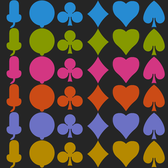
\includegraphics[scale = 0.8]{images/Spielsteine}
	\caption{Alle möglichen Farbe/Form Kombinationen der Spielsteine}
	\label{fig:Spielsteine}
\end{figure}

Von jeder Kombination gibt es genau drei Steine im Spiel, also insgesamt 108 Spielsteine. Alle Spielsteine werden zu Beginn des Spiels gemischt und im Spielsteinbeutel abgelegt. Die nächsten 12 Spielsteine, welche aus dem Beutel gezogen werden können, werden unterhalb des Beutels angezeigt. Die Nummer auf dem Beutel gibt die Anzahl, der sich noch im Beutel befindenden Spielsteine an. Hierbei ist zu beachten, dass damit die Gesamtanzahl der Spielstein im Vorrat gemeint ist. Sowohl die nicht einsehbaren, als auch die schon sichtbaren Spielsteine unterhalb des Beutels.\\

\begin{figure}[h] \centering 
	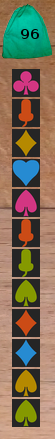
\includegraphics[scale = 0.7]{images/Vorratsbeutel}
	\caption{Der Vorratsbeutel}
	\label{fig:Vorratsbeutel}
\end{figure}
Jeder Spieler besitzt zu Beginn und am Ende eines jeden Zuges immer genau 6 Steine in seinem Vorrat, wobei auch der Vorrat des gegnerischen Spieler eingesehen werden kann.\\


\section{Spielablauf}		
	Es beginnt der rote Spieler. Jeder Spieler hat in seinem Zug zwei verschiedene Möglichkeiten. Entweder er legt einen oder mehrere Spielsteine auf dem Spielbrett aus, oder er tauscht 1-6 seiner Spielsteine gegen Neue ein.	
	
\subsection{Spielsteine auslegen}
Beim Anlegen gelten folgende Regeln:
\begin{itemize}
\item Zwei oder mehr Steine nebeneinander bilden eine Reihe.
\item Eine Reihe besteht entweder aus Spielsteinen welche die gleich Farbe oder die gleiche Form besitzen.
\item In einer Reihe von gleichen Formen darf jede Farbe nur genau einmal vorkommen.
\item In einer Reihe von gleichen Farben darf jede Form nur genau einmal vorkommen.
\item Eine Reihe besteht somit aus maximal 6 Spielsteinen.
\item Ein Spielstein der ausgelegt werden soll muss immer an schon vorhandene Spielsteine angelegt werden. Ausnahme ist hier der als erstes ausgelegte Spielstein einer Partie. Dieser darf beliebig auf dem Spielbrett platziert werden.
\item Wenn ein Spielstein an eine bereits existierende Reihe angelegt wird, so muss dieser zu den jeweiligen Eigenschaften dieser Reihe passen.
\item In jedem Zug dürfen Spielsteine an genau einer Reihe angelegt werden. Die Reihe darf in jede der beiden Richtungen erweitert werden.
\end{itemize}

Nach dem Anlegen der Spielsteine wird der Vorrat des Spielers wieder auf 6 Steine aus dem Beutel aufgefüllt. Die Steine die dieser erhält, können in der Reihe unterhalb des Beutels eingesehen werden. Der Spielstein, welcher sich ganz unten befindet ist der erste, der gezogen wird.\\
Um einen Stein anzulegen, klickt man auf diesen und zieht ihn auf das Spielbrett. Wenn eine mögliche Position angewählt wurde, wird das Spielfeld grün unterlegt. Ansonsten wird das Spielfeld rot unterlegt. Um alle bisher gelegten Steine zurück in den Vorrat zu holen klickt man auf den Button \emph{Steine zurücknehmen}. Um seinen Zug zu beenden und die momentan auf dem Spielbrett liegenden Steine fest anzulegen klickt man auf den Button \emph{Steine legen}.
	 
\subsection{Spielsteine tauschen}
Kann ein Spieler keine Spielsteine anlegen oder ist er mit seinem Vorrat unzufrieden, so besteht die Möglichkeit 1-6 Spielsteine gegen Neue aus dem Beutel zu tauschen. Er erhält dann die von ihm gewählte Anzahl von Spielsteinen aus den offen liegenden Spielsteinen. Seine abgegebenen Steine werden zurück in den Beutel getan, welcher danach gemischt wird.\\
Nach dem Tausch ist der Zug des Spielers beendet.\\
Zum Tauschen, klickt man die gewünschte Anzahl von Steinen an. Diese werden dann durch einen grünen Rahmen umrandet. Um den Tausch zu Vollziehen, klickt man auf den Button \emph{Steine tauschen}. Um die Auswahl aufzuheben kann man jeden Stein einzeln anklicken, oder auf den Button \emph{Steine zurücknehmen} klicken. Sind Spielsteine zum Tausch ausgewählt, ist es nicht möglich einen Stein auf dem Spielbrett auszulegen.
	
\subsection{Punkteverteilung}
Das Tauschen von Spielsteinen bringt 2 Punkte, unabhängig davon, wie viele Steine getauscht werden.\\
Beim Anlegen von Spielsteinen erhält man für jeden Stein, der sich in einer erweiterten Reihe befindet einen Punkt. Ein Stein wird doppelt gezählt, wenn er Teil von zwei Reihen ist.\\
Wenn man es schafft eine Reihe von 6 Steinen zu vervollständigen bildet man ein \textbf{Sixpack}. Für diesen Stein erhält man 6 Punkte für jeden Stein der Reihe und außerdem einen Bonus von 6 Punkten, also insgesamt 12 Punkte.
TODO: Beispielbilder zur Wertung.
	
\section{Ende des Spiels}
Das Ende des Spiels tritt in zwei Fällen auf. Im regulären Fall endet es nach 25 Runden. Der zweite Fall tritt auf, sobald ein Spieler in einem Zug so viele Steine legt, dass er seinen Steinevorrat nicht mehr komplett aus dem allgemeinen Vorrat auffüllen kann. Dieser Spieler erhält noch seine Punkte aus diesem Zug und Unmittelbar anschließend ist das Spiel beendet. Legt ein Spieler beispielsweise 4 Steine an, während sich nur noch 3 Steine im Sack befinden, so ist das Spiel nach diesem Zug vorbei.\\
Der Spieler mit den meisten Punkten gewinnt. Haben beide Spieler die gleiche Anzahl an Punkten, so gibt es ein Unentschieden.

\subsection{Spezialfall: Keine Züge mehr möglich}
Sollte der Fall eintreten, dass keine Spielsteine mehr angelegt werden können, so müssen die Spieler Steine tauschen, bis die maximale Rundenanzahl erreicht ist. Dieser Fall kann auftreten wenn ein 6 mal 6 Quadrat gelegt wurde (siehe Abbildung  ~\ref{fig:Spielsteine}).
	
\section{Die graphische Benutzeroberfläche}
\subsection{Übersicht der graphischen Benutzeroberfläche}
TODO
	
\subsection{Das Einstellungsmenü}
	 \begin{figure}[h]
		\centering
		%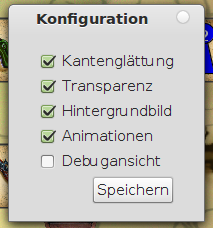
\includegraphics[scale=0.5]{bilder/configuration}
		\caption{Das Einstellungsmenü}
		\label{fig:Configuration}
	\end{figure}
	
	Ein Einstellungsmenü mit Darstellungsoptionen lässt
sich über die Leertaste anzeigen. Dazu muss das
Spielfeld den Tastaturfokus haben (erforderlichenfalls
vorher Mausklick auf das Spielfeld). Es stehen dort
folgende Einstellungen zur Verfügung:

\textbf{Kantenglättung} und \textbf{Transparenz} verbessern die Optik des
Spiels, sind jedoch rechenintensiv. Auf sehr langsamen Rechnern sollten sie daher
deaktiviert werden. \textbf{Hintergrundbild} ist zwar weniger rechenintensiv,
kann aber auch aus Gründen der Übersichtlichkeit deaktiviert werden.\\
\textbf{Animationen} legt fest, ob die Bewegungen der Spielsteine in
Wiederholungen und bei Computerspielern animiert werden sollen.\\
Die \textbf{Debugansicht} verkleinert die Punkteanzeige in der Seitenleiste
etwas und zeigt unterhalb Debug-Hilfestellungen zu einzelnen Zügen an. Diese
Hilfestellungen sind Texte, die ein Spielclient einem Zug beifügen kann, den er
an den Spielserver sendet.
	
\end{document}
